
\section{绪论/Introduction}

微波技术是 20 世纪初发展起来的,特别是第二次世界大战中雷达的研制加速了微波技术的发展,使其成为一门独立的学科。它主要研究的对象是微波。微波是一种频率非常高的电磁波,它在电磁波谱中占有很小的波段范围,如图 1 所示。

\begin{figure}[htbp]
	\centering
	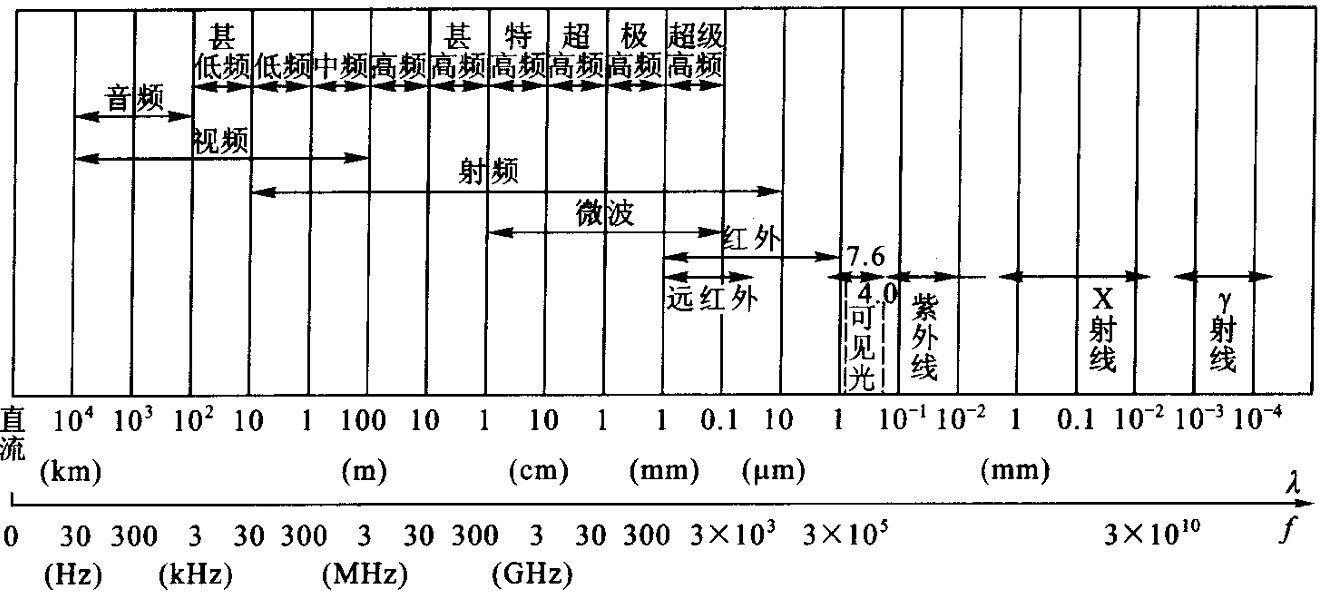
\includegraphics[width=0.8\textwidth]{img/1-1.png} % 图片文件名,不需要加扩展名
	\caption{微波频段示意图 \cite{chen2019artificial}}
	\label{fig:example}
\end{figure}

微波的定义:把波长在 1m - 0.1mm 范围内的电磁波称为微波。微波波段对应的频率范围为:
\( 3 \times 10^8 \sim 3 \times 10^{12} \, \text{Hz} \)
。在整个电磁波谱中,微波处于普通无线电波与红外线之间(包含了远红外部分),是频率最高的无线电波,它的频带宽度比所有普通无线电波波段总和宽约 10000 倍。一般情况下,微波又可划分为分米波、厘米波、毫米波和亚毫米波四个波段。

\subsection{微波的特性}
与普通无线电波相比,微波具有如下四个主要特性。

1.似光性

微波波长短,它的波长比地球上的宏观物体(如建筑物、飞机和军舰等)的尺寸小得多,其传播特性与光相似:沿直线传播、遇到障碍物时会产生反射。利用这一特点,可以制造出高方向性微波天线,用来发射或接收微波信号。从而为雷达、微波中继通信、卫星通信和导弹制导等提供了必要条件。

2.频率高

与普通无线电波相比,微波的频率要高得多,在同样的相对带宽条件下,微波的可用绝对带宽特别宽,能容纳的信息容量很大。因此,微波可作为多路通信的载频。另外,微波受外界干扰小、且不受电离层变化的影响,故通信质量高于普通无线电波。

由于微波的频率高,其振荡周期(10 −9 ∼10 −12s)与低频器件电子的渡越时间(一般为 10 −9s)属同一个数量级。因此,低频波段时可以忽略的一些物理现象,如极间电容、引线电感、集肤效应和辐射效应等,在微波波段特别明显,必须加以考虑。此外,传输微波的电路是一种分布参数电路,所使用的器件是特殊的微波器件。

3.能穿透电离层

利用本身的高频振荡,微波可以穿透电离层。由于微波不能被电离层所反射,所以微波的地面通信只限于天线的视距范围之内,远距离微波通信需要用中继站接力。但另一方面,利用微波能穿透电离层这一特点,又可以进行宇航通信、卫星通信和射电天文学研究等,因此微波开辟了电磁波谱中的一个“宇宙窗口”。

4.量子特性

微波具有波粒二象性。根据量子学理论,电磁辐射的能量不是连续的,而是由一个个的“能量子”组成,每个量子具有与其频率成正比的能量 E = hf)(其中 (f 为频率,普朗克常数 h=6.626×10 −34
J·s)。低频无线电波的频率很低,量子能量甚小,故其量子特性不明显。而微波的频率很高,其量子能量范围大约在 10 −5∼10 −2eV,故在低功率电平下,微波的量子特性明显地表现出来。另外,一些分子和原子的超精细结构能级落在微波波段,顺磁物质在磁场作用下的能级差也落在这一波段。利用微波与这些物质相互作用产生的物理现象,可用以研究物质的结构,从而形成一门“微波波谱学”。微波与物质的相互作用比较强烈,特别是水分子吸收了微波能量后会产生热效应,这一特点在实际中可以充分利用。

\subsection{微波技术的研究方法}
微波技术的基本理论是经典的电磁场理论,研究电磁波沿传输线的传播特性有两种分析方法。一种是“场”的分析方法,即从麦克斯韦方程出发,在特定边界条件下解电磁波动方程,求得场量的时空变化规律,分析电磁波沿线的各种传输特性;另一种是“路”的分析方法,即将传输线作为分布参数电路处理,用基尔霍夫定律建立传输线方程,求得线上电压和电流的时空变化规律,分析电压和电流的各种传输特性。事实上,“场”和“路”的分析方法是紧密相关的,很多方面两者相互补充。

因为在微波领域中所有的电磁现象都是随时间和空间而变化的物理过程,有的宜用“路”的方法处理,因此电路理论中的许多概念和方法在这里同样具有重要的地位。另一些电磁现象却宜用“场”的方法。有时对同一电磁现象既可用“路”的方法,也可用“场”的方法,两种方法只是分析同一问题的不同途径。

\subsection{微波技术的应用}
微波技术的实际应用相当广泛,尤其近年来随着它的发展,新的应用层出不穷。这里简单介绍几种主要应用。

1.在雷达方面的应用

雷达是微波技术的早期应用,事实上,正是由于第二次世界大战期间对于雷达的需要,微波技术才迅速发展起来。雷达设备可以利用微波信号准确地测定目标的方向、距离和速度,从而对运动目标实现定位、跟踪和识别。目前,用于军事上的有制导雷达、跟踪雷达、警戒雷达和炮瞄雷达等;用于民用上的有导航雷达、气象雷达和遥感雷达等。

2.在通信方面的应用

由于微波频带宽,信息容量大,因此微波可用于多路通信。在有线通信方面,利用同轴电缆可以同时传送几千路电话和几路电视信号;在无线通信方面,利用微波的中继接力传送电视信号,利用微波能穿透电离层的特性,可进行卫星通信和宇航通信,利用外层空间三颗互成 120 ∘角的同步卫星,就能实现全球通信和电视实况转播。

3.医学与生物工程

微波治疗:微波被用于肿瘤治疗(如微波消融术)和皮肤病的治疗。
生物传感:微波技术用于检测生物组织的电磁特性,帮助诊断疾病。
药物合成:微波辅助化学反应加速药物合成过程。



